% 英文で執筆する場合はクラスファイルへのオプションを[T,E]としてください.
% If you want to write your paper in English, pass to [T,E] options to document class.
\documentclass[T,J]{fose} % 「コンピュータソフトウェア」用のクラスファイルは compsoft です.
\taikai{2024} % 固定です.出版委員長が毎年変更してAuthor Kitを配布してください.

\usepackage [dvipdfmx] {graphicx}

% ユーザが定義したマクロなどはここに置く.ただし学会誌のスタイルの
% 再定義は原則として避けること.

% 以下は説明のために使用したパッケージであるため,削除可能.
\usepackage{listings}
\usepackage{tabularx}
\usepackage{fancyvrb}
\usepackage{xurl}
\usepackage{cite}
\usepackage[dvipdfmx]{graphicx}
\usepackage{latexsym}
\usepackage[T1]{fontenc}
\usepackage{lmodern}
\usepackage{textcomp}
\usepackage{latexsym}
\usepackage{url}
\usepackage{longtable}
\usepackage{multirow}
%\usepackage{color}
\usepackage{xcolor}
\usepackage{colortbl}
%\usepackage[noadjust]{cite}

\newcommand{\todo}[1]{\colorbox{yellow}{{\bf TODO}:}{\color{red} {\textbf{[#1]}}}}
\newcommand{\change}[1]{\colorbox{green}{{\bf CHANGE}:}{\color{black} {\textbf{[#1]}}}}
\newcommand{\new}[1]{\colorbox{cyan}{{\bf NEW}:}{\color{black} {\textbf{[#1]}}}}
\newcommand{\rqone}{リリースまでの期間に応じて検証/導入されるチケットの特徴に違いがあるか?}
\newcommand{\rqtwo}{リリースまでの期間に応じて優先的に検証/導入されるチケットの変化をどの程度捉えられるか?}
\newcommand{\rqthree}{\todo{rq}}

% 以下のマクロはサンプルファイル作成用のマクロです.不要であれば削除してください.
\newcommand{\foseclassfile}{fose.cls}
\newcommand{\fosestylefile}{fose.sty}


\begin{document}

% 論文のタイトル
\title{リリースまでの期間に応じて優先的に検証/導入されるコードレビューチケットの特徴分析}
% 以下の \etitle(と\@etitle)はFOSE論文フォーマット独自のマクロです.
% FOSEに投稿した論文を発展させてコンピュータソフトウェアに投稿される場合はコメントアウトしてください.
% \setetitleは奇数ページのヘッダに表示する文字列(\etitle)を設定するためのマクロです.
% タイトルが2行に渡る場合は "\\" を 使用することで任意の位置で改行をすることができます.
\setetitle{Prioritized Analysis of Reviewed or Merged Review Tickets for Each Periods before Release}
%\setetitle{Long Long Long Long Long Long \\ Long Long Long Long Long \\ Long Long Long Long Long Long Long Long Long Long Long Long Paper Title}

% タイトル,著者などが複数行にわたり,論文冒頭の著者名が日本語アブストと重複して描画された場合に以下のコメントアウトを外してください.
%\longtitle

% 著者
% 和文論文の場合,姓と名の間には半角スペースを入れ,
% 複数の著者の間は全角スペースで区切る
%
\author{上中 瑞稀 伊原 彰紀
%
% ここにタイトル英訳 (英文の場合は和訳) を書く.
% 英語タイトルは論文1ページ目左下,著者らの名前・所属一覧の一番上に表示される
%
% 上記\setetitle中で改行した場合は "\etitle" を削除し,改行(\\)を入れていないタイトルを記載してください.
% \ejtitleは1ページ目左下に挿入されるタイトルとして使用されます.
% また,"\etitle"はFOSE論文フォーマット独自のマクロです.
\ejtitle{\etitle}
\shozoku{Mizuki Uenaka, Akinori Ihara}{和歌山大学}
{Wakayama University}
}

%
% 和文アブストラクト
% In English paper, content of Jabstract will be ignored. 
\Jabstract{%
オンラインコードレビューサービスを導入するOSS開発では,日々多くのコードレビューを依頼するコードレビューチケットが提出され,検証者は優先的にコードレビューするチケットを選択する.従来研究では,チケット提出時に得られる特徴に基づき優先順位づけする手法が提案されているが,コードレビューするチケットの優先順位は日々変動する.本研究では,直近のリリースまでの期間に応じて検証/導入されるコードレビューチケットの特徴の違いを分析する.また,リリースまでの期間別に優先的に検証/導入されるコードレビューチケットを予測する.ケーススタディとして,OpenStackプロジェクトを対象に分析した結果,リリースまでの期間に応じて検証/導入されるチケットの特徴には違いがあることを明らかにした.また,優先的に検証/導入されるコードレビューチケットを予測した結果,特に終期において提案手法の有用性が示された.
%ソフトウェア開発において,コードレビューはソフトウェアの品質維持のために重要な役割を担っているが,時間と作業量ともに高いコストを要する.従来研究では,コードレビューの依頼時に作成されるチケットから計測できる特徴に基づき,開発者らが優先的に検証するチケットを特定する手法を提案している.しかし,急を要さない不具合修正やリファクタリングの変更提案に関するチケットを検証する優先順位は日々変動する.本研究では,直近のリリースまでの期間に応じて検証/導入されるコードレビューチケットの特徴の違いを分析する.また,リリースまでの期間別に優先的に検証/導入されるコードレビューチケットを予測する.ケーススタディとして,OpenStackプロジェクトのコアコンポーネント6プロジェクトを対象に分析した結果,直近のリリースまでの期間に応じて検証/導入されるコードレビューチケットの特徴が違うことを明らかにした.また,予測結果から特にリリース直前において提案モデルの有用性が示された.
}
%
\maketitle \thispagestyle {empty}


%%%%%%%%%%%%%%%%%%%%%%
\section{はじめに}
%%%%%%%%%%%%%%%%%%%%%%

ソフトウェア開発において,変更提案されたソースコードの可読性や欠陥の有無を開発者が評価するコードレビューの作業は,ソフトウェアの品質維持のために重要な役割を担っている~\cite{quality1}\cite{quality2}.コードレビューでは,複数人の開発者(検証者)がソースコードを検証し,ソースコードを実装した開発者(実装者)と共にソースコード変更の妥当性について合意形成を図り,必要に応じて修正を繰り返す.

コードレビューはソフトウェア開発プロセスの一連の作業において,時間,作業量ともに高いコストを要する作業である\cite{cost}.コードレビューを効率化するため,昨今ではGitHub,Gerrit,Review Boardなどのオンラインコードレビューサービスを利用した方式(モダンコードレビュー\cite{quality1})の導入が増加している.このようなサービスではソースコードの変更提案をレビューチケットとして保存・管理する.大規模なソフトウェア開発プロジェクトでは,日々膨大なソースコードの変更提案が提出されており,
%Gerritを使用するNovaプロジェクトでは一日平均10件\todo{多く見えない...1人あたりにする?またはレビューが多いって言ってる論文を引用する?}のチケットが作成されている.
検証者は変更提案の内容や緊急性を考慮しながら優先的に検証するチケットを選択している\cite{integrator}.

%2章にこういう文章書いてますがどうでしょう
%1つのコードレビューチケットの確認に数日から数ヶ月の期間を要することもあり,1週間で平均6時間程度をコードレビューに費やすプロジェクトも多い\cite{review2}.
%-> ここはチケット数の説明の方がわかりやすい気がする

従来研究では,チケット提出時に得られる特徴(変更行数や変更ファイル数など)に基づき,開発者らが優先的に検証するチケットを機械学習アルゴリズムを用いて特定する手法を提案している\cite{prioritizer}\cite{review_prioritize_pineapple}.
%\change{追加した2つ目の従来研究ですが,1日ごとにチケットの情報を持ってきて優先順位付けしていたので,若干違いますが\todo{他に従来研究があれば追記}ということだったので,一旦入れています}
当該手法は,セキュリティに関連するようなソフトウェア利用者に悪影響を与えるソースコードの改善のように,チケット提出時期によって優先順位の変動が小さいチケットの特定に有用である.
%急を要さない不具合修正,リファクタリングの変更提案に関する
しかし,検証する優先順位が日々変動するチケットが存在する.Kononenkoらは,開発者へのインタビューにおいて,直近のリリースに導入するチケットの優先順位はリリースまでの期間によって異なることを明らかにしている\cite{release_merge}.特に,ラピッドリリースを導入しているプロジェクトでは検証を次のリリースに延期することも少なくない.従来手法は,このようなリリースまでの期間などの開発状況に応じた検証するチケットの優先順位の決定には適していない.

% ける直近のリリースまでの期間や変更提案におけるコードレビューの進捗度,同時期にコードレビューに取り組む変更提案数などの開発状況が考慮されない.しかし,他の従来研究\cite{release_merge}では,直近のリリースに導入する変更提案の優先順位はリリースまでの期間によって異なることが開発者へのインタビューから示唆された.

%個々の変更提案に対する開発者の関心を捉えるモデルを開発することで,開発者がすぐに関心を持つ変更提案に対して優先順位付けを行っている.\todo{ここ以降のこの段落の訂正}この従来研究の手法では,予測時点における直近のリリースまでの期間や変更提案におけるコードレビューの進捗度,同時期にコードレビューに取り組む変更提案数などの開発状況が考慮されない.しかし,他の従来研究\cite{release_merge}では,直近のリリースに導入する変更提案の優先順位はリリースまでの期間によって異なることが開発者へのインタビューから示唆された.
%また,検証者数や検証者の専門性などの開発リソースに応じて,コードレビューの対象とできる変更提案には限りがある.


%\change{\todo{導入を見る動機も書きたい}により次の一文を改変したい}
本研究では,直近のリリースまでの期間に応じて検証されるコードレビューチケットの特徴の違いを明らかにする.さらに,リリースまでの期間別に優先的に検証されるコードレビューチケットを予測する有効性を明らかにする.また,従来研究\cite{estimate_merge_time}ではコードレビューに要する時間はチケットの特徴に限らず,チケット提出時期の開発状況にも依存するため,本研究では直近のリリースまでの期間に応じて導入されるコードレビューチケットも分析する.本研究では,コードレビューツールGerritを使用するクラウド基盤ソフトウェアOpenStackの6つのコアコンポーネントプロジェクトを対象に2つのリサーチクエスチョン (RQ) を検証する.

\noindent\textbf{RQ1: \rqone}\\
%\change{完全に従来研究から引っ張ってきたわけでは無いため,文章を書き換え}
RQ1では,従来研究\cite{prioritizer}で提案されている開発者やチケットの特徴(4種類)と従来研究\cite{review1}\cite{release_merge}の知見から有用と示唆される開発者や変更内容の特徴(3種類)を特徴量として計測し,リリースまでの期間別に検証/導入されるコードレビューチケットの特徴量の違いを分析する.

\noindent\textbf{RQ2: \rqtwo}\\
RQ2では,RQ1で計測した特徴量を用いてチケットが直近のリリースに検証/導入されるか否かを予測するモデルをリリースまでの期間別に構築し,評価する.また従来研究との比較として分析対象期間を区別しないモデルによる予測結果と比較する.
%コードレビューが行われる変更提案や,直近にリリースされるバージョンに導入する変更提案を予測する機械学習モデルを構築する.また,全期間のデータセットを混ぜたモデルを構築し,それぞれの予測精度を比較する.

%\noindent\textbf{RQ3: \rqthree}\\

以降,本論文では,\ref{sec:intro}章でOSS開発におけるコードレビュープロセスと従来研究について述べる.その後,\ref{sec:dataset}章で分析対象とするデータセットを述べ,\ref{sec:rq1},\ref{sec:rq2}章でRQ1,RQ2の分析手法および結果を述べる.そして,\ref{sec:disc}章で結果の考察を述べる.\ref{sec:validity}章で妥当性について述べ,\ref{sec:fig-tab-exp}章でまとめる.

%%%%%%%%%%%%%%%%%%%%%%
\section{ソフトウェア開発におけるコードレビュープロセス}\label{sec:intro}
%%%%%%%%%%%%%%%%%%%%%%

\subsection{コードレビュープロセス}
%コードレビューは高品質なソフトウェアをリリースするために,ソースコードの可読性や欠陥の有無を検証する作業である.
図\ref{fig:codereviewprocess}はコードレビュー作業の一連の流れを説明する概略図を示す.検証者は,実装者が提出したコードレビューチケットを確認し,変更提案に対して3つの判断(導入,却下,修正要求)のいずれかを決定する.導入はソースコードをリポジトリに導入し,却下はソースコードを導入することなくコードレビューチケットを閉じる.修正要求は,コードレビューチケットを提出した実装者にソースコードの改修を依頼する.検証者は,修正要求を繰り返すことで,ソフトウェアの品質を維持しつつ,不具合修正やさらなる機能拡張を行う.

コードレビューはソフトウェア開発に多大な貢献をもたらす一方で,膨大なコストがかかる作業でもある.1つのコードレビューチケットの確認に数日から数ヶ月の期間を要することもあり,1週間で平均6時間程度をコードレビューに費やすプロジェクトも多い\cite{review2}.特に,大規模なオープンソースソフトウェア (OSS) 開発では,膨大なチケットを受け付けるため,検証者は変更提案の内容や緊急性を考慮して,優先的に検証するチケットを選択している\cite{integrator}.

%-----------------------
\begin{figure}[t]
\begin{center}
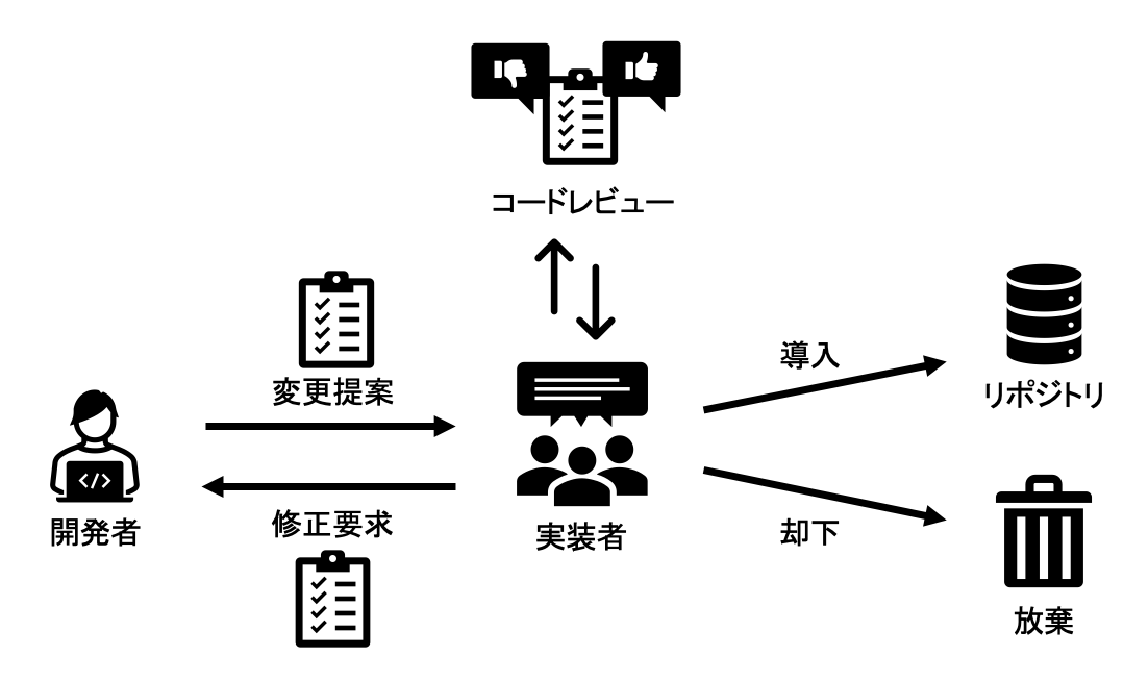
\includegraphics[width=1.0\linewidth]{Uenaka_fig/code_review_process.pdf}
\caption{コードレビュープロセス}
\label{fig:codereviewprocess}
\end{center}
\end{figure}
%-----------------------

\subsection{従来研究}
%\change{全体的に文章を書き換え.1つ目は全期間モデルをベースラインとするため,2,3つ目は特徴量の説明として必要があるため,記述しています.}

\subsubsection{チケットの優先順位付け}
Veen\cite{prioritizer}らは,OSS開発を対象にコードレビューの優先順位付け手法を提案している.従来研究では,機械学習アルゴリズムを用いて,変更内容や作成者の特徴などの14種類の特徴を説明変数とし,コードレビューチケットに翌日までに検証結果が投稿されるか否かを予測する手法を提案している.当該研究ではリリースまでの期間によって日々優先順位が変動するような変更提案のチケットに対して誤った優先順位を算出することが示唆される.そのため,本研究ではリリースまでの期間ごとに予測モデルを構築し,ベースラインと比較することでリリースまでの期間による予測精度の違いを分析する.

%¥begin{table}[t]
%  ¥caption{従来研究¥cite{prioritizer}で用いる14種類の説明変数}
%  ¥label{table:juurai}
%  ¥centering
%  ¥vspace{0.5zh}
%  ¥begin{tabular}{l|lr}
%    ¥hline
%    ¥multicolumn{1}{c|}{説明変数}  & ¥multicolumn{1}{|c}{説明}  ¥¥
%    ¥hline ¥hline
%    経過時間  & 変更提案が提出されてからの経過分数 ¥¥
%    貢献率  & 変更提案作成者のプロジェクトでのコミット率 ¥¥
%    受入率  & 変更提案作成者が過去に提出した変更提案の導入率 ¥¥
%    追加行数  &  変更提案で追加されている変更行数 ¥¥
%    削除行数  & 変更提案で削除されている変更行数  ¥¥
%    リビジョン数  & 変更提案のリビジョン数 ¥¥
%    ファイル数  & 変更提案の変更ファイル数 ¥¥
%    コメント数 & 変更提案のコメント数 ¥¥
%    レビュー数  &  変更提案に対してのコードレビュー数 ¥¥
%    コアメンバー  & 変更提案の作者はプロジェクトメンバーか ¥¥
%    ブランチ  & 変更コードとマージ先のリポジトリが同一か ¥¥
%    issue含有  & 変更提案に紐づいているissueがあるか ¥¥
%    最終コメント &  最終コメントでユーザがメンションされているか ¥¥
%    テストコード含有  & 変更ファイルにテストコードが含まれているか ¥¥
%    ¥hline
%  ¥end{tabular}
%¥end{table}


\subsubsection{開発者の貢献量がチケットの検証/導入判断にもたらす影響}
Bosu\cite{review1}らは,OSS開発における開発者の地位がチケットの導入に影響するのか否かを明らかにするために,OSS開発に積極的に貢献する開発者と消極的な開発者がそれぞれ作成したソースコードのレビュープロセスの違いに関する調査を行なった.8つのOSSプロジェクトから導入もしくは却下と判断されたチケットのコードレビューデータを調査した結果,積極的に貢献する開発者のチケットほど,導入もしくは却下までの時間が短く,導入される確率が高いことが明らかとなった.そのため本研究では,実装者の貢献量を捉えるため,従来研究\cite{prioritizer}の特徴量である導入実績(実装者が過去に提案したチケットの導入率)だけでなく,報告実績(実装者が過去に提案したチケット数)を特徴量に加え,リリースまでの期間ごとの特徴量の違いを分析する.

\subsubsection{変更内容がチケットの検証判断にもたらす影響}
Kononenko\cite{release_merge}らは,コードレビューにかかる時間および導入判断に影響を与える要因を明らかにするためにコードレビューチケットを調査している.定性的分析として開発者へのインタビューを行った結果,レビューにかかる時間は変更内容(バグ修正,リファクタリング等)によって異なることが明らかとなった.そのため,本研究では変更内容によって検証判断が異なると考え,従来研究\cite{bug}\cite{refactoring}において利用されていたパターンをチケットのタイトルと概要に適用することで,バグ修正確信度とリファクタリングを特徴量に加え,リリースまでの期間ごとの特徴量の違いを分析する.

\subsection{本研究の動機}
従来研究\cite{prioritizer}は,優先順位の変動が小さいコードレビューチケットの特定には有用であるが,リリースまでの期間に検証の優先順位が変化するチケットの選択には適していない.しかし,提出されるチケット数,検証可能な開発者数のような開発リソースによって,検証/導入可能なチケット数が異なることが示唆される.本研究では,RQ1としてリリースまでの期間に着目し,リリースまでの期間別に検証/導入されるコードレビューチケットの特徴を分析する.RQ2では,RQ1で分析した特徴量を用いてリリースまでの期間別に,優先的に検証/導入されるコードレビューチケットを予測する.


%直近のバージョンリリースまでの期間やその時点での対応可能な開発者数などの開発状況は考慮されていない.しかし,ソフトウェア開発において,バージョンリリースが近い場合は新たに提出された大規模な変更を導入するためにコードレビューのリソースを割く時間が無いというように,開発状況によって対応する変更提案は異なると考える.そこで,RQ1では,開発状況の中でもリリースまでの期間に着目し,リリースまでの期間に応じた検証/導入される変更提案の特徴を分析することで,開発状況によって対応する変更提案は異なるという仮説の検証を行う.また,RQ2では,RQ1で分析した特徴量を用いてリリースまでの期間ごとに検証/導入される変更提案の予測を行うことで,リリースまでの期間ごとの予測精度の評価を行う.


%%%%%%%%%%%%%%%%%%%%%%%%%%%%%%%%%%%%%%%%%%
\section{分析対象データセット}\label{sec:dataset}
%%%%%%%%%%%%%%%%%%%%%%%%%%%%%%%%%%%%%%%%%%
%\change{またGitHubから〜の一文を書き換えるとともに,プロジェクトごとの変更提案数の表が削除されて辻褄が合わなくなっていた箇所の訂正を行いました.}
本研究では,OpenStackプロジェクトのうち,コアコンポーネント6プロジェクト(Nova,Neutron,Cinder,Keystone,Swift,Glance)を分析対象とする.各プロジェクトの変更提案の中で,立ち上げ時から2022年9月時点で導入もしくは却下されたコードレビューチケットを収集する.具体的には,OpenStackがコードレビュー管理システムとして使用するGerrit\footnote{Gerrit: \url{https://review.opendev.org}}から,コードレビュー履歴を収集し,変更提案のチケットの特徴量を計測した.またGitHubから,各バージョンのリリース日およびリリースに導入されたチケットの特定を行った.
%\todo{どうやって?従来研究は?要引用}
分析対象プロジェクトのリリース間隔が約3ヶ月であるため,本研究では各プロジェクトでリリースに導入されたコードレビューチケットの変更提案を対象とし,特にリリース直前の3ヶ月に導入されたチケット数の上位5バージョンを分析対象とする.表\ref{table:release}は分析対象とする各プロジェクトのバージョンを示す.また,長期間に渡り放置される変更提案は,短期的な優先順位の決定には関与しないため,
%分析結果のノイズとなり得るため,
リリース直前の6ヶ月以内に提出されたチケットを分析対象とする.

%->todo2 柏さんからいただいたコミットの親子関係を辿るプログラムを使って,親子関係を辿ることでリリースに導入されたチケットの特定を行っています.<- 柏先生も共著に入れればよかった...まぁ論文誌で.ちなみに,引用は聞いておいた方が良くない?柏先生を共著に入れられていないことも含めて.論文誌でお願いしますと連絡しておいては?
%明日朝に連絡します.すみません.

%-------------------
% \begin{table}[t]
% \centering
%   \caption{プロジェクトごとの変更提案数}
%   \vspace{0.5zh}
%   \label{table:henkou}
%   \begin{tabular}{l|r}  \hline \hline
%     \multicolumn{1}{c|}{プロジェクト} & \multicolumn{1}{c}{変更提案数} \\ \hline
%     Nova & 39,870 \\ 
%     Neutron & 24,467 \\ 
%     Cinder & 17,155 \\
%     Keystone & 10,764 \\ 
%     Swift & 8,737 \\ 
%     Glance & 6,248 \\ \hline
%   \end{tabular}
% \end{table}

%------------------------
\begin{table*}[t]
\centering
  \caption{プロジェクトごとの対象リリースバージョン}
  \vspace{0.5zh}
  \label{table:release}
  \scalebox{0.88}{
  \begin{tabular}{l|r|l}  \hline \hline
    プロジェクト &チケット数 & \multicolumn{1}{c}{バージョン(リリース3ヶ月以内に導入されたチケット数 )}\\ \hline 
    Nova & 39,870 & 13.0.0.0b3(529),14.0.0.0b1(475),16.0.0.0b2(451),17.0.0.0b1(410),20.0.0.0rc1(392)\\ 
    Neutron & 24,467 & 7.0.0.0b1(326),8.0.0.0b1(400),9.0.0.0b1(296),11.0.0.0b1(286),16.0.0.0b1(186)\\ 
    Cinder & 17,155 & 8.0.0.0b1(249),8.0.0.0rc1(249),9.0.0.0b2(249),11.0.0.0b2(249),12.0.0.0b2(235)\\ 
    Keystone & 10,764 & 8.0.0a0(182),9.0.0.0b3(211),10.0.0.0b2(220),11.0.0.0b1(167),15.0.0.0rc1(165)\\ 
    Swift & 8,737 & 1.9.2(180),2.4.0(154),2.7.0(117),2.17.0(105),2.27.0(101)\\ 
    Glance & 6,248 & 11.0.0a0(70),12.0.0.0b1(83),12.0.0.0b3(72),13.0.0.0b1(64),17.0.0.0b1(73)\\ \hline
  \end{tabular}
  }
\end{table*}



%%%%%%%%%%%%%%%%%%%%%%
\section{RQ1: \rqone}\label{sec:rq1}
%%%%%%%%%%%%%%%%%%%%%%

\subsection{分析手法}
%\change{図\ref{fig:labeling}に合わせて文章を一部書き換え,図\ref{fig:labeling}のラベルは検証->検証開始済み,導入->導入済みに直した方がいいですか?3分ぐらいでできます}
\subsubsection{コードレビューチケットの分類}
本研究では,リリースまでの3ヶ月の期間内に検証/導入されるコードレビューチケットの特徴量の違いを明らかにする.具体的には,各プロジェクトのリリース間隔が約3ヶ月(12週間)であるため,リリース直前の12週間を図\ref{fig:labeling}に示すように12週前から8週前までを初期,8週前から4週前までを中期,4週前からリリースまでを終期として4週間ずつの3期間に分割し,それぞれの期間において優先的に検証されたチケットの特徴量の違い(RQ1-1),および優先的に導入されたチケットの特徴量の違い(RQ1-2)をそれぞれ分析する.

\textbf{(RQ1-1 検証)} 本研究では各期間において,従来研究\cite{prioritizer}と同様に,検証者からのコメントや評価が投稿されれば優先的に検証されるチケットと捉え「検証開始済み」と分類し,チケットの提出から検証を開始するまでは「非検証」に分類する.本研究では,時期に応じて優先的に検証を要すると判断されるチケットの特徴を明らかにするため,すでに検証を要すると判断された「検証開始済み」のチケットは,次の期間以降から分析対象外とする.したがって,図\ref{fig:labeling}では,初期に提出されたチケットは検証されていないため「非検証」に分類する.次に中期に検証者からのコメントや評価が投稿されたため「検証開始済み」に分類する.

\textbf{(RQ1-2 導入)} 本研究では各期間において,GitHubリポジトリにマージ処理されると「導入済み」に分類し,チケットの提出からリポジトリにマージ処理されるまでは「非導入」に分類する.また「導入済み」のチケットは,次の期間以降から分析対象外とする.したがって,図\ref{fig:labeling}では,初期に提出されたチケットは導入されていないため「非導入」に分類する.次に終期にマージ処理されたため「導入済み」に分類する.


% のように,変更提案に対して2週間ごとに検証/非検証および導入/非導入のラベル付けを行う.直近のリリースに向けて優先的に検証/導入される変更提案の特徴がリリースまでの期間によって異なるかを明らかにするため,12週間前から4週間ごとに最初にコードレビューされるまでは非検証のラベル,コードレビューされたときは検証のラベルを付与する.また,導入するか否かが決定されるまでは非導入のラベル,決定された時は導入もしくは非導入のラベルを付与する.

% RQ1では,多数の変更提案の中から優先される変更提案の特徴を分析する.そこで,10週間前〜8週間前では優先的に検証された変更提案に対して,8週間前〜6週間前では優先的に検証されないとして非検証のラベルを付与することは,分析時のノイズとなる可能性があるため,図\ref{fig:labeling}の変更提案においては,優先的に検証された10週間前〜8週間前以降は検証/非検証のラベル,優先的に導入された4週間前〜2週間前以降は導入/非導入のラベルを付与しないこととする.

%-----------------------
\begin{figure}[t]
\begin{center}
\scalebox{1.3}{
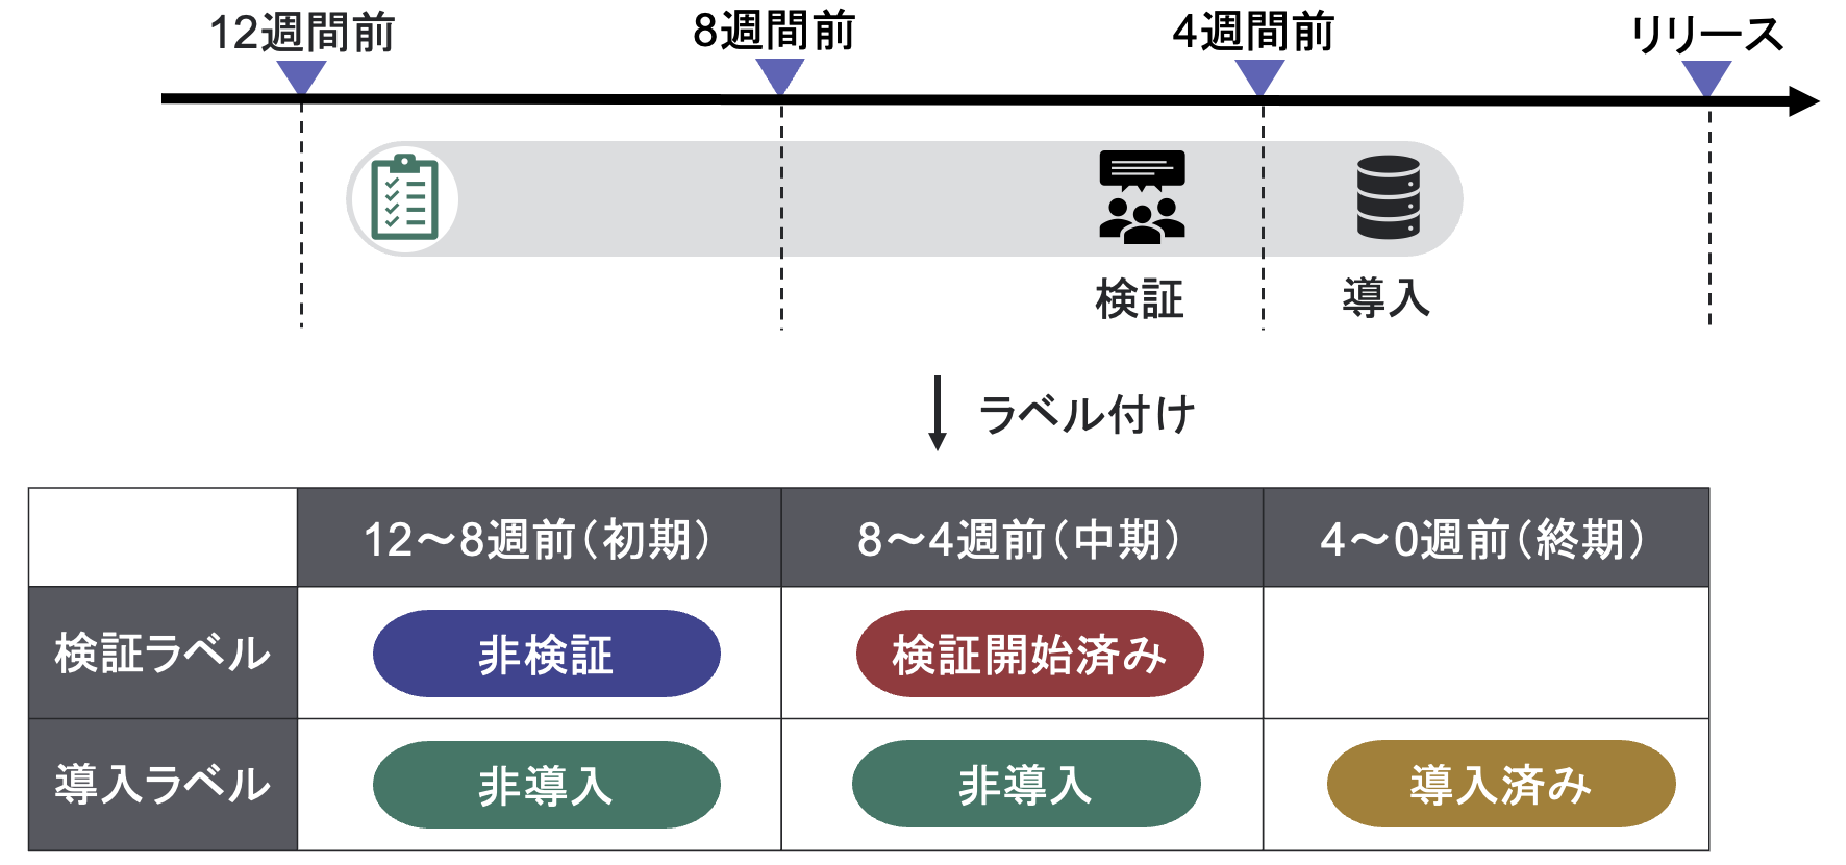
\includegraphics[width=0.8\linewidth]{Uenaka_fig/labeling.pdf}
}
\caption{ラベル付け}
\label{fig:labeling}
\end{center}
\end{figure}
%-----------------------


\subsubsection{レビューチケットの特徴量の計測}
本研究では,表\ref{table:metrics}に示す7種類の特徴量をリリースまでの各期間における分析対象のチケットから計測する.これらの特徴量は,従来研究に基づき決定した特徴量である.ただし,従来研究で計測していたGitHub特有の説明変数は計測対象外とする.
%\change{\todo{バグ修正確信度の説明はしておいた方が良くないですか?}により次の文を追加.}
バグ修正確信度は,従来研究\cite{bug}においてCVSのログメッセージに適用されていたパターンをチケットのタイトルと概要に適用することで,チケットがバグである確度を3値に分類した特徴量である.
%一応2.2.3で軽くは触れているのですが,やはり詳細な説明必要ですよね..<-はい,そう思います.従来研究はあくまで位置付けや立ち位置の説明で,方法を説明する場所ではないので,ここで説明しておいた方が安全だと思います. <- やります
%を対象としてコミット率の\todo{コミット率って何?}ような特徴量を計測していたが,本研究ではGerritを用いるため,計測しない.
なお,本研究では報告実績等の時系列によって値が変化する特徴量は,同一の変更提案でもリリースまでの期間別に再計測する.

%本論文では,検証者が容易に取得できる情報から特徴量を収集したいと考えたため,主にGerritにおいて変更提案が一覧に列挙されているリスト群等から収集を行なった.

%-----------------------
\begin{table}[t]
  \caption{RQ1の分析に用いる7種類の特徴量}
  \label{table:metrics}
  \centering
  \vspace{0.5zh}
    \scalebox{0.65}{
  \begin{tabular}{l|l|l}
    \hline \hline
    \multicolumn{1}{c|}{特徴量}  & \multicolumn{1}{c|}{説明}  & \multicolumn{1}{c}{従来研究}  \\
    \hline
    報告実績  & 実装者が過去に提案したチケット数  & \cite{review1} \\
    導入実績  & 実装者が過去に提案したチケットの導入率  & \cite{review1},\cite{prioritizer} \\
    追加行数  &  チケットで追加されている変更行数  & \cite{prioritizer},\cite{diff} \\
    削除行数  & チケットで削除されている変更行数  & \cite{prioritizer},\cite{diff}  \\
    テストコード含有  & 変更ファイルにテストが含まれているか  & \cite{prioritizer} \\
    バグ修正確信度  &  バグ修正の変更提案である確度  & \cite{bug},\cite{release_merge} \\
    リファクタリング  & リファクタリングの変更提案か否か  & \cite{refactoring},\cite{release_merge} \\
    \hline
  \end{tabular}
  }
\end{table}
%-----------------------

\subsubsection{レビューチケットの特徴量の比較}
初期,中期,終期の3つの期間における検証/導入されるコードレビューチケットの特徴量を分析する.具体的には,リリースまでのそれぞれの期間において,未検証チケットと検証開始済みチケット,また導入チケットと非導入チケットに関する特徴量の違いをそれぞれマンホイットニーのU検定を用いて統計的有意差を確認する.

%--------------------
\begin{table*}[t]
\caption{RQ1-1:検証される変更提案と検証されない変更提案の特徴量の検定結果\\(Nova(No),Neutron(Ne),Cinder(C),Keystone(K),Swift(S),Glance(G))}
\label{table:review_notreview_prepare}
\centering
\vspace{0.5zh}
\scalebox{0.76}{
\begin{tabular}{l|cccccc|cccccc|cccccc}
    \hline \hline
    \multirow{2}{*}{特徴量} & \multicolumn{6}{c|}{初期} & \multicolumn{6}{c|}{中期} & \multicolumn{6}{c}{終期} \\ \cline{2-19}
    & No & Ne & C & K & S & G & No & Ne & C & K & S & G & No & Ne & C & K & S & G \\ \hline
    導入実績 & *** & *** &  &  &  & *** & *** & *** & * & ** &  & *** & *** & *** & *** & *** &  & *** \\
    報告実績 &   &  & ** & *** &   & ** &   &   & *** & *** & * &   &  & *** &  &  &  *** &  \\
    追加行数 & *** & *** & * & *** & *** & *** & *** & *** & *** & *** & *** & *** & *** & *** & *** & *** & *** & *** \\
    削除行数 & * & *** &  &  & ** &   &  & * &   &   & *** &   &   &  & ** &  &   &  \\
    テストコード含有 & *** &  &  & *** &   &   & *** &   &   &   &   & * &  & ** & * & * &   &  \\
    バグ修正確信度 & *** & *** & *** & ** &  & *** & *** & *** & *** &  &   & ** & *** & *** & *** & * &   & *** \\
    リファクタリング &  &  &  & ** &   &  &   & * & ** &  &   &  &  &   & ** &    &   &  \\ \hline
\end{tabular}}


\vspace{2mm}
\caption{RQ1-2:導入される変更提案と導入されない変更提案の特徴量の検定結果\\(Nova(No),Neutron(Ne),Cinder(C),Keystone(K),Swift(S),Glance(G))}
\label{table:merge_notmerge_prepare}
\centering
\vspace{0.5zh}
\scalebox{0.76}{
\begin{tabular}{l|cccccc|cccccc|cccccc}
    \hline \hline
    \multirow{2}{*}{特徴量} & \multicolumn{6}{c|}{初期} & \multicolumn{6}{c|}{中期} & \multicolumn{6}{c}{終期} \\ \cline{2-19}
    & No & Ne & C & K & S & G & No & Ne & C & K & S & G & No & Ne & C & K & S & G \\ \hline
    導入実績 & *** & *** & *** & *** & *** & *** & *** & *** & *** & *** & *** & *** & *** & *** & *** & *** & *** & *** \\
    報告実績 & *** & *** & *** & *** & * & *** & *** & *** & *** & *** &   & * & *** & *** & *** & *** &  &  \\
    追加行数 & *** & *** & *** & * & *** & * & *** & *** & *** & *** & *** & *** & *** & *** & *** & *** & *** & *** \\
    削除行数 &   & ** &  &  &  &   &   &   & ** &   &   &   &   &    &   &  & * & ** \\
    テストコード含有 & *** & *** &  & *** &   & *** & *** & *** & *** & *** & * & ** & *** & *** &  & ** & ** &    \\
    バグ修正確信度 & *** & *** & *** &   &   &  *  & *** & *** & *** & *** & ** & *** & *** & *** &    & * &   & *** \\
    リファクタリング & *** &   & ** &   &  *  & ** &   &   &   &   &   & * & ** &   &   &    & ** & * \\ \hline
\end{tabular}}
\end{table*}
%--------------------

\subsection{結果}
RQ1では,リリースまでの期間(初期,中期,終期)に応じて,検証開始済み/非検証のチケットや導入済み/非導入のチケットの特徴量に対してマンホイットニーのU検定を用いることで,チケットの特徴量を比較する.結果の表では,P値が0.01未満は***,0.01〜0.05は**,0.05〜0.1は*で表記する.

\textbf{(RQ1-1 検証)} 表\ref{table:review_notreview_prepare}は,各プロジェクトの初期,中期,終期において検証されるチケットと検証されないチケットの特徴量の検定結果を示す.表\ref{table:review_notreview_prepare}の結果から,多くのプロジェクトにおいて追加行数の特徴量はいずれの期間でも検証開始済み/非検証のチケット間で統計的に有意な差があることを確認した.次に,導入実績は初期と比べて中期や終期で統計的に有意差を確認できた.図\ref{fig:review_notreview}は,リリースが近づくにつれ統計的な有意差を確認できたCinderプロジェクトの未検証チケットと検証開始済みチケットの導入実績の分布を示す.リリースが近づくにつれて未検証チケットと検証開始済みチケットをそれぞれ作成した開発者の導入実績の差が顕著になり,導入実績の高い開発者が作成したチケットが優先的に検証されていることが示唆される.したがって,リリースまでの期間に応じて検証されるチケットの特徴には違いがあることが示唆された.


%-----------------------
\begin{figure}[t]
\begin{center}
\scalebox{1.0}{
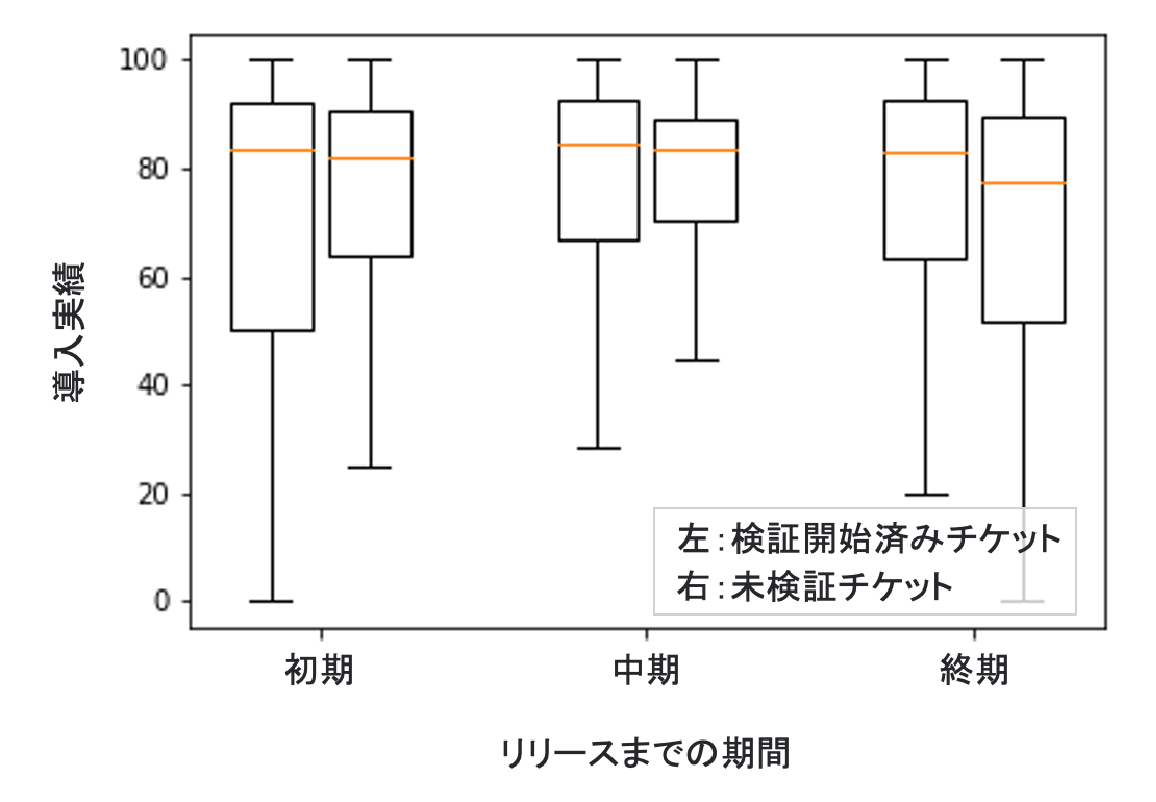
\includegraphics[width=0.8\linewidth]{Uenaka_fig/review_notreview.pdf}
}
\caption{Cinderプロジェクトにおける検証開始済み/非検証のチケットの導入実績の分布}
\label{fig:review_notreview}
\end{center}
\end{figure}
%-----------------------

%-----------------------
\begin{figure}[t]
\begin{center}
\scalebox{1.0}{
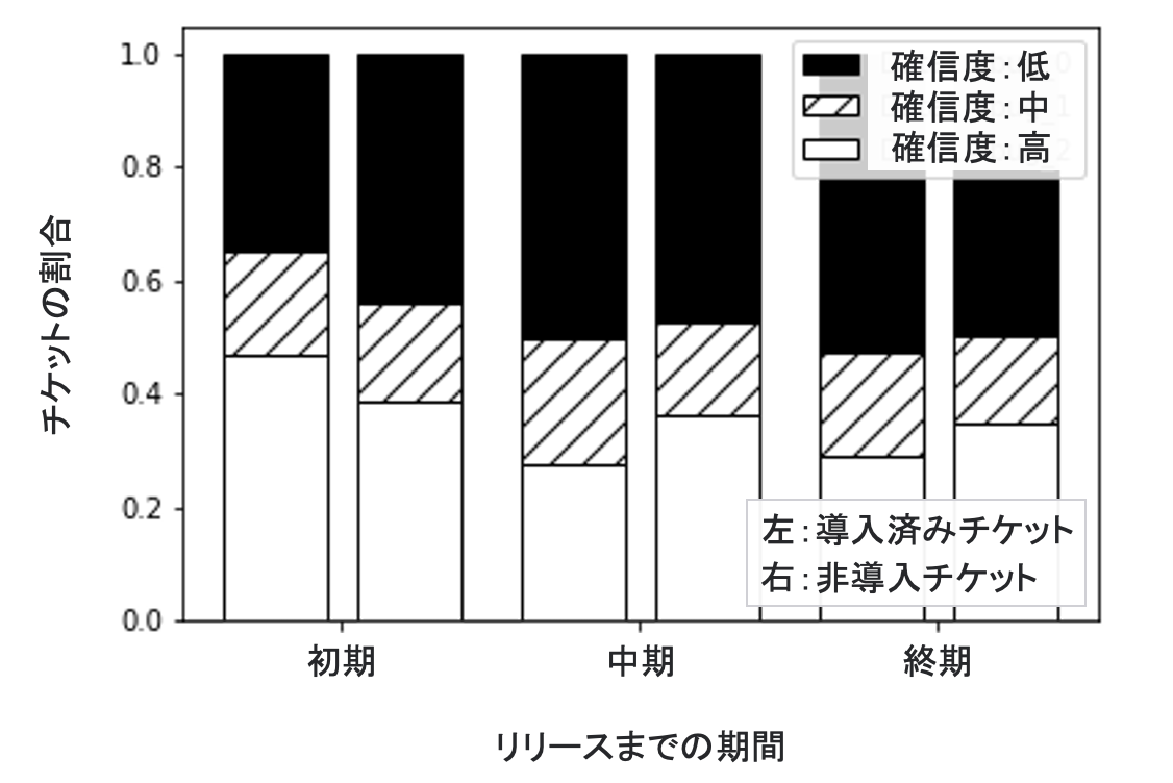
\includegraphics[width=0.8\linewidth]{Uenaka_fig/merge_notmerge.pdf}
}
\caption{Keystoneプロジェクトにおける導入済み/非導入のチケットのバグ修正確信度の分布}
\label{fig:merge_notmerge}
\end{center}
\end{figure}
%-----------------------

\textbf{(RQ1-2 導入)} 表\ref{table:merge_notmerge_prepare}は各プロジェクトの初期,中期,終期において導入されるチケットと導入されないチケットの特徴量の検定結果を示す.表\ref{table:merge_notmerge_prepare}の結果から,導入実績,追加行数の特徴量は全てのプロジェクトの全期間において,導入済み/非導入のチケット間で統計的に有意な差があった.一方,バグ修正確信度は初期や終期と比べて中期の方が統計的に有意差のあるプロジェクトが増加する.図\ref{fig:merge_notmerge}にリリースまでの期間によって有意差の変化したKeystoneプロジェクトの導入済みチケットと非導入チケットのバグ修正確信度の分布を示す.バグ修正確信度は提案がバグ修正である確度を3値に分類した特徴量であり,図\ref{fig:merge_notmerge}では黒色で示されている提案が最もバグである確度が低く,次いで斜線,白色と図\ref{fig:merge_notmerge}の積み上げ棒グラフの下部の分類ほどバグである確度が高い.この結果から,特に中期ではバグ修正確信度の低いチケットが優先的に導入されるという結果が得られた.
%\change{\todo{終期でも同じような結果だけど,有意差はないので,これ言えるかな?}により次の文章を追記}
なお,終期も中期と同じような結果であるが,これは終期のバグ修正確信度にも導入済み/非導入のチケット間で統計的に有意な差があったためであると考えられる.したがって,リリースまでの期間に応じて導入されるチケットの特徴には違いがあることが示唆された.

% これでも一番有意な差があるように見えるものを引っ張っております..他の特徴量も考慮した上でこれです<- Keystoneでは終期でも有意差あるってこと書いておいてもいいかもね. <- 確かにその方がむしろ結果が妥当っぽいですかね

\textbf{(結果のまとめ)} RQ1-1,1-2の分析結果から,リリースまでの期間に応じて検証/導入されるチケットの特徴には違いがあることが示唆された.


%%%%%%%%%%%%%%%%%%%%%%%%%%%%%%%%%
\section{RQ2: \rqtwo}\label{sec:rq2}
%%%%%%%%%%%%%%%%%%%%%%%%%%%%%%%%%
\subsection{分析手法}

\subsubsection{予測モデルの構築}
%\change{図\ref{fig:predict_schematic}引用してるし,こっちのセクションでベースラインの全期間モデルについて触れるか悩み中.気持ちとしては評価するためのモデルなので評価のセクションで触れるのがベストかな...と.}
RQ2では,直近のリリースまでに検証されるか否か,直近のリリースまでに導入されるか否かを目的変数とする2クラス分類モデル(検証予測モデル,導入予測モデル)を期間別に構築する.図\ref{fig:predict_schematic}は,予測モデルを構築するための概略図を示す.本研究では初期モデル,中期モデル,終期モデルの3モデルを構築し,ベースライン手法として初期,中期,終期の全ての期間のデータセットを用いて学習および評価を行う全期間モデルを構築する.具体的には,5バージョンのうち最も新しい1つをテストデータとし,残り4つを学習データとすることで各モデルを構築する.
検証予測モデルおよび導入予測モデルの構築には,それぞれ機械学習アルゴリズムであるRandom Forestsモデル\cite{randomforest}を用いる.しかし,RQ2では目的変数が不均衡なデータを扱うため,Balanced Random Forestsモデル\footnote{imblearn.ensemble.BalancedRandomForestClassifier: \url{https://imbalanced-learn.org/stable/references/generated/imblearn.ensemble.BalancedRandomForestClassifier.html}}を用いる.

%-----------------------
\begin{figure}[t]
\begin{center}
\scalebox{1.25}{
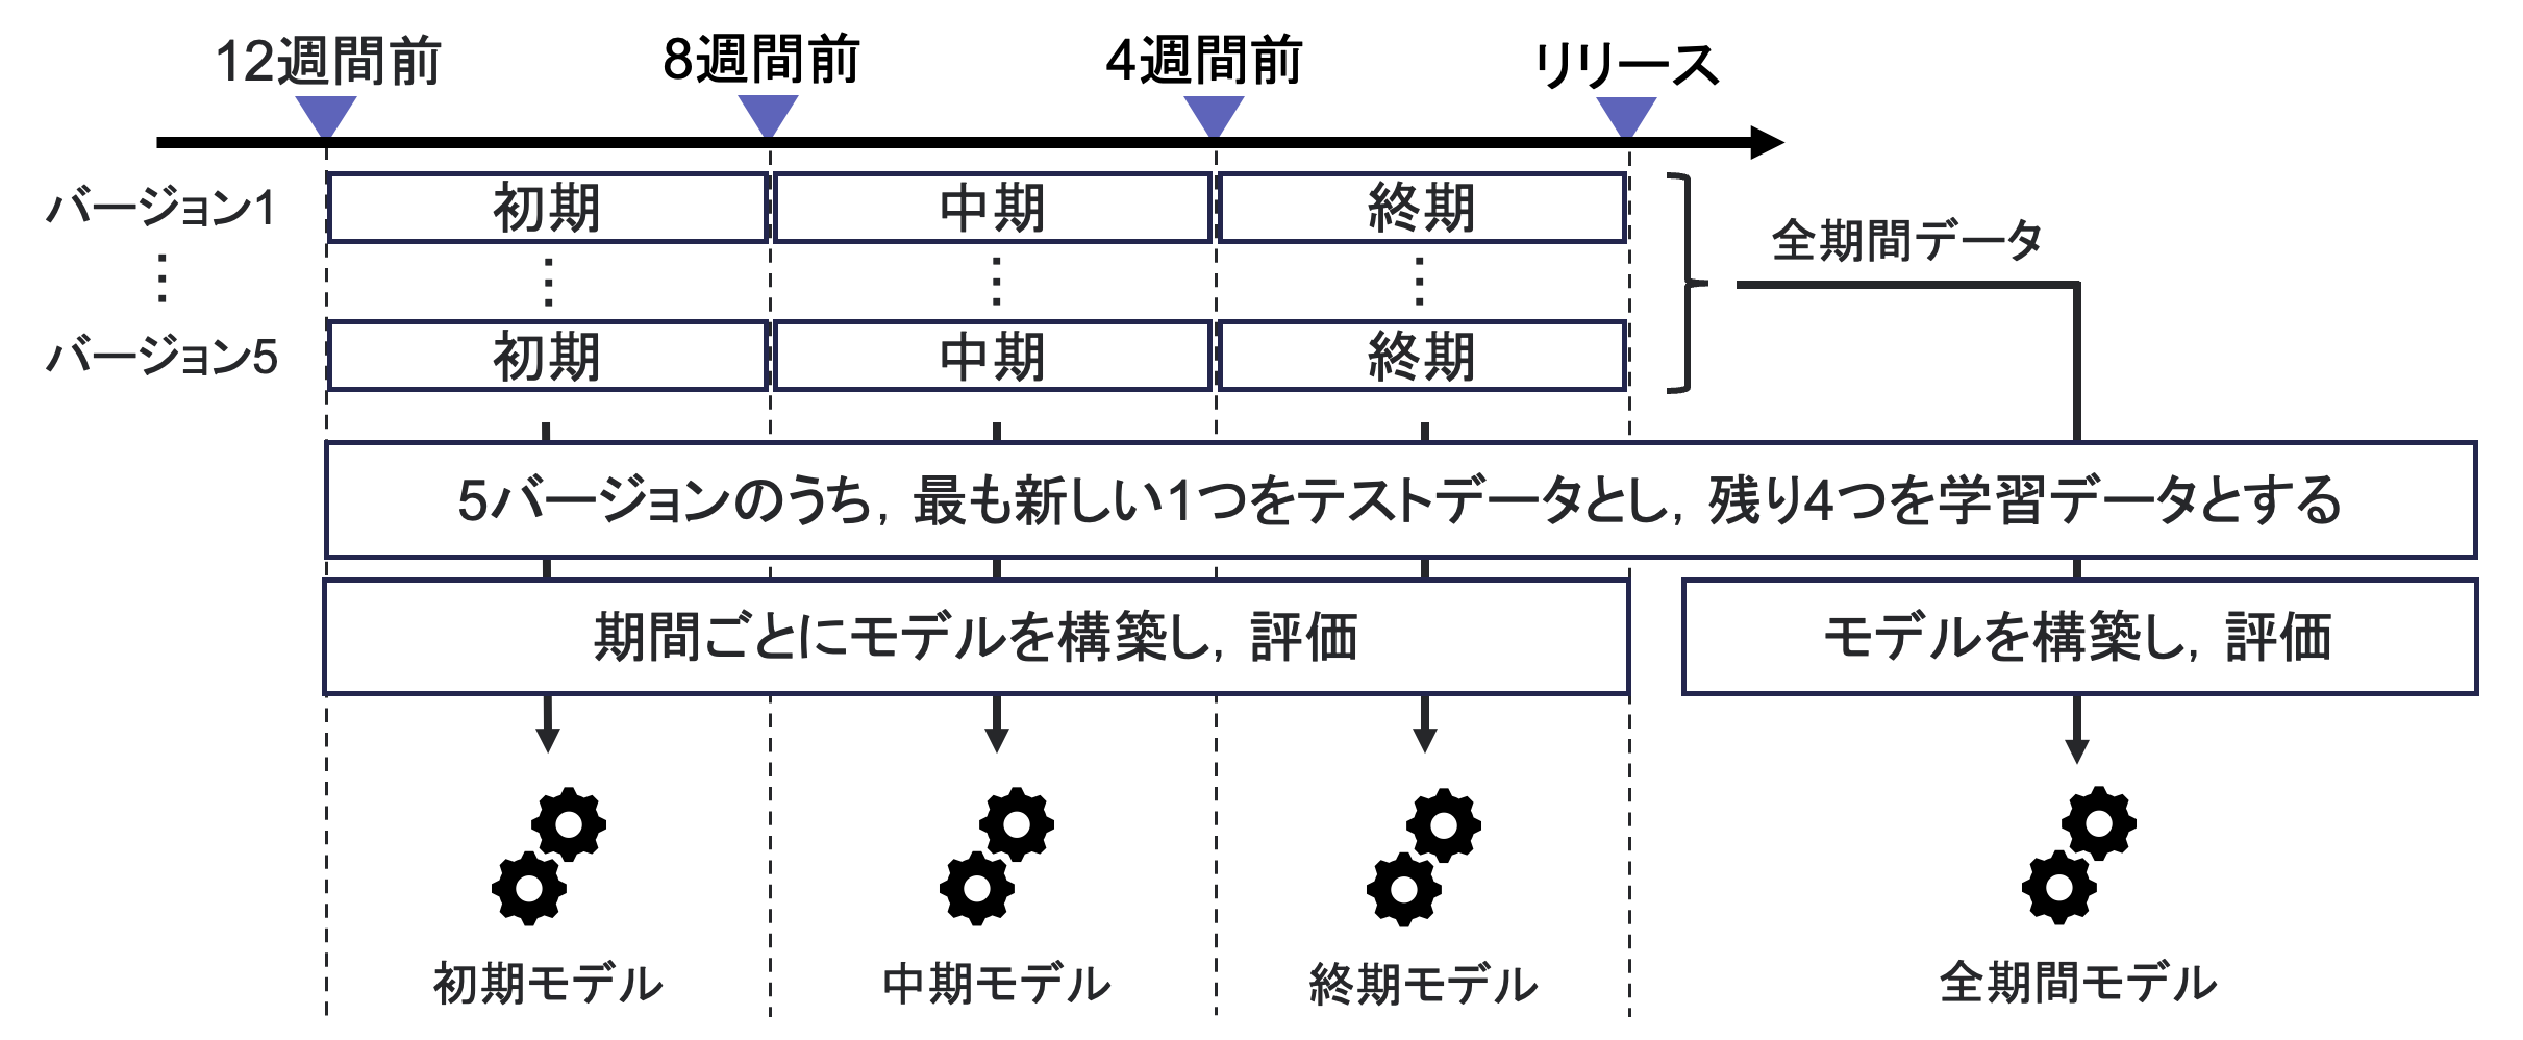
\includegraphics[width=0.8\linewidth]{Uenaka_fig/predict_schematic.pdf}
}
\caption{予測モデル構築の概略図}
\label{fig:predict_schematic}
\end{center}
\end{figure}
%-----------------------

\subsubsection{予測モデルの評価}
%\change{全体的に図\ref{fig:predict_schematic}に合うように書き換え.特に〜以降は\todo{適合率か再現率のどちらを優先するのか,また場合によっては適合率の意味を説明すべきかもしれない.}に合わせて書き換えています.どうでしょう?あとaccuracy載せる必要ないと思い,消しています(Veen\cite{prioritizer}らの従来研究で指標になっていたのとシンプルな正解率もあっていいかと思っていたため載せていた).}
%図\ref{fig:predict_schematic}のように,期間ごとに学習および評価を行うモデルとして,
初期モデル,中期モデル,終期モデル,全期間モデルは,評価指標として適合率,再現率,F値を用い,提案手法の予測精度とベースライン手法の予測精度を比較する.評価指標のうち,適合率はモデルが正例(検証するまたは導入する)と予測したうちの正解割合,再現率は正解のうちモデルが正例と予測した割合であり,この2つの指標はトレードオフの関係である.本研究では,ベースライン手法は期間を問わない汎用性の高いモデルが構築される一方,提案手法は学習するデータをリリースまでの期間で区切っているため,その期間に特化したモデルが構築されると考える.従って,提案手法では再現率よりも適合率が高くなると考え,適合率とF値を対象に予測結果を解釈する.

\subsection{結果}
表\ref{table:review_predict}は検証予測モデル,表\ref{table:merge_predict}は導入予測モデルの結果を示す.
それぞれ,提案手法とベースライン手法を比較して精度の高いモデルを太字で表記する.また,提案手法の中で最も高い精度の背景色を灰色で示す.

\textbf{(RQ2-1 検証)} 表\ref{table:review_predict}の結果から,提案手法とベースライン手法の精度を比較すると適合率は初期モデルでは2プロジェクトで2\%〜5\%向上し,4プロジェクトで6\%〜19\%低下した.中期モデルでは4プロジェクトで3\%〜10\%向上し,2プロジェクトで5\%〜15\%pt低下した.終期モデルでは5プロジェクトで1\%〜20\%向上し,1プロジェクトで12\%低下した.また,F値は初期モデルでは1プロジェクトで3\%向上し,5プロジェクトで12\%〜19\%低下した.中期モデルでは6プロジェクト全てで8\%〜17\%低下した.終期モデルでは4プロジェクトで1\%〜7\%向上し,2プロジェクトで3\%〜15\%低下した.この結果から,終期モデルは半数以上のプロジェクトで適合率およびF値が全期間モデルより高い精度であるため,特に終期において提案手法の有用性が示された.
%\change{\todo{残り半数は考察で述べるなら,考察で述べると書いておいた方がいい.}により追記}なお,終期モデルの精度が提案手法の中で最も低くなったGlanceプロジェクトについては\ref{secsec:glance_review}章で考察を述べる.


%-------
\begin{table*}[t]
\caption{RQ2-1:検証モデルの予測結果}
\label{table:review_predict}
\centering
  \scalebox{0.88}{
\begin{tabular}{l|rrrr|rrrr|rrrr}
    \hline \hline
    \multirow{3}{*}{評価指標} & \multicolumn{4}{c|}{Nova} & \multicolumn{4}{c|}{Neutron} & \multicolumn{4}{c}{Cinder} \\ \cline{2-13}
    & \multicolumn{3}{c}{提案手法} & \multicolumn{1}{c|}{ベース} & \multicolumn{3}{c}{提案手法} & \multicolumn{1}{c|}{ベース} & \multicolumn{3}{c}{提案手法} & \multicolumn{1}{c}{ベース} \\ \cline{2-13}
    & \multicolumn{1}{l}{初期} & \multicolumn{1}{l}{中期} & \multicolumn{1}{l}{終期} & \multicolumn{1}{l|}{全期間} & \multicolumn{1}{l}{初期} & \multicolumn{1}{l}{中期} & \multicolumn{1}{l}{終期} & \multicolumn{1}{l|}{全期間} & \multicolumn{1}{l}{初期} & \multicolumn{1}{l}{中期} & \multicolumn{1}{l}{終期} & \multicolumn{1}{l}{全期間} \\ \hline 
%    正確率 & 0.50 & 0.53 & {\textbf{0.57}} & 0.56 & 0.50 & 0.53 & 0.57 & {\textbf{0.58}} & 0.53 & 0.58 & {\textbf{0.71}} & 0.67 \\ 
    適合率 & 0.44 & \cellcolor{lightgray}{\textbf{0.56}} & \cellcolor{lightgray}{\textbf{0.56}} & 0.53 & 0.57 & 0.61 & \cellcolor{lightgray}{\textbf{0.72}} & 0.66 & {\textbf{0.84}} & \cellcolor{lightgray}{\textbf{0.89}} & {\textbf{0.83}} & 0.82 \\ 
    再現率 & 0.54 & 0.52 & \cellcolor{lightgray}0.68 & {\textbf{0.80}} & 0.51 & 0.55 & \cellcolor{lightgray}0.61 & {\textbf{0.64}} & 0.49 & 0.57 & \cellcolor{lightgray}{\textbf{0.77}} & 0.74 \\ 
    F値 & 0.48 & 0.54 & \cellcolor{lightgray}0.61 & {\textbf{0.64}} & 0.53 & 0.57 & \cellcolor{lightgray}{\textbf{0.66}} & 0.65 & 0.62 & 0.69 & \cellcolor{lightgray}{\textbf{0.80}} & 0.78 \\ \hline        
    \multirow{1}{*}{プロジェクト名} & \multicolumn{4}{c|}{Keystone} & \multicolumn{4}{c|}{Swift} & \multicolumn{4}{c}{Glance} \\ \hline
%    & \multicolumn{3}{c}{提案手法} & \multicolumn{1}{c|}{ベース} & \multicolumn{3}{c}{提案手法} & \multicolumn{1}{c|}{ベース} & \multicolumn{3}{c}{提案手法} & \multicolumn{1}{c}{ベース} \\ \cline{2-13}
%    & \multicolumn{1}{l}{初期} & \multicolumn{1}{l}{中期} & \multicolumn{1}{l}{終期} & \multicolumn{1}{l|}{全期間} & \multicolumn{1}{l}{初期} & \multicolumn{1}{l}{中期} & \multicolumn{1}{l}{終期} & \multicolumn{1}{l|}{全期間} & \multicolumn{1}{l}{初期} & \multicolumn{1}{l}{中期} & \multicolumn{1}{l}{終期} & \multicolumn{1}{l}{全期間} \\ \hline \hline
%    正確率 & {\textbf{0.56}} & {\textbf{0.52}} & {\textbf{0.63}} & 0.52 & 0.47 & {\textbf{0.58}} & {\textbf{0.65}} & 0.58 & {\textbf{0.75}} & 0.64 & 0.58 & 0.73 \\ 
    適合率 & 0.47 & {\textbf{0.63}} & \cellcolor{lightgray}{\textbf{0.73}} & 0.53 & 0.38 & \cellcolor{lightgray}{\textbf{0.66}} & \cellcolor{lightgray}{\textbf{0.66}} & 0.57 & \cellcolor{lightgray}{\textbf{0.88}} & 0.68 & 0.71 & 0.83 \\ 
    再現率 & 0.57 & 0.38 & \cellcolor{lightgray}0.67 & {\textbf{0.79}} & 0.58 & 0.49 & \cellcolor{lightgray}{\textbf{0.79}} & 0.75 & \cellcolor{lightgray}{\textbf{0.81}} & 0.78 & 0.63 & 0.81 \\ 
    F値 & 0.51 & 0.47 & \cellcolor{lightgray}{\textbf{0.70}} & 0.64 & 0.46 & 0.57 & \cellcolor{lightgray}{\textbf{0.72}} & 0.65 & \cellcolor{lightgray}{\textbf{0.85}} & 0.73 & 0.67 & 0.82 \\ \hline                      
\end{tabular}
}

\vspace{4mm}

\caption{RQ2-2:導入モデルの予測結果}
\label{table:merge_predict}
\centering
  \scalebox{0.88}{
\begin{tabular}{l|rrrr|rrrr|rrrr}
    \hline \hline
    \multirow{3}{*}{評価指標} & \multicolumn{4}{c|}{Nova} & \multicolumn{4}{c|}{Neutron} & \multicolumn{4}{c}{Cinder} \\ \cline{2-13}
    & \multicolumn{3}{c}{提案手法} & \multicolumn{1}{c|}{ベース} & \multicolumn{3}{c}{提案手法} & \multicolumn{1}{c|}{ベース} & \multicolumn{3}{c}{提案手法} & \multicolumn{1}{c}{ベース} \\ \cline{2-13}
    & \multicolumn{1}{l}{初期} & \multicolumn{1}{l}{中期} & \multicolumn{1}{l}{終期} & \multicolumn{1}{l|}{全期間} & \multicolumn{1}{l}{初期} & \multicolumn{1}{l}{中期} & \multicolumn{1}{l}{終期} & \multicolumn{1}{l|}{全期間} & \multicolumn{1}{l}{初期} & \multicolumn{1}{l}{中期} & \multicolumn{1}{l}{終期} & \multicolumn{1}{l}{全期間} \\ \hline 
%    正確率 & 0.52 & 0.57 & 0.57 & {\textbf{0.62}} & 0.56 & {\textbf{0.64}} & 0.55 & 0.57 & {\textbf{0.62}} & {\textbf{0.54}} & {\textbf{0.60}} & 0.52 \\ 
    適合率 & 0.15 & {\textbf{0.27}} & \cellcolor{lightgray}{\textbf{0.31}} & 0.27 & 0.27 & \cellcolor{lightgray}{\textbf{0.38}} & 0.28 & 0.31 & 0.09 & {\textbf{0.26}} & \cellcolor{lightgray}{\textbf{0.39}} & 0.24 \\ 
    再現率 & \cellcolor{lightgray}{\textbf{0.74}} & {\textbf{0.73}} & 0.52 & 0.60 & 0.44 & \cellcolor{lightgray}{\textbf{0.69}} & 0.55 & 0.58 & 0.33 & 0.54 & \cellcolor{lightgray}0.57 & {\textbf{0.62}} \\ 
    F値 & 0.26 & \cellcolor{lightgray}{\textbf{0.40}} & {\textbf{0.39}} & 0.37 & 0.33 & \cellcolor{lightgray}{\textbf{0.49}} & 0.37 & 0.40 & 0.15 & {\textbf{0.35}} & \cellcolor{lightgray}{\textbf{0.46}} & 0.35 \\ \hline                      
    \multirow{1}{*}{プロジェクト名} & \multicolumn{4}{c|}{Keystone} & \multicolumn{4}{c|}{Swift} & \multicolumn{4}{c}{Glance} \\ \cline{2-13}
    % & \multicolumn{3}{c}{提案手法} & \multicolumn{1}{c|}{ベース} & \multicolumn{3}{c}{提案手法} & \multicolumn{1}{c|}{ベース} & \multicolumn{3}{c}{提案手法} & \multicolumn{1}{c}{ベース} \\ \cline{2-13}
    % & \multicolumn{1}{l}{初期} & \multicolumn{1}{l}{中期} & \multicolumn{1}{l}{終期} & \multicolumn{1}{l|}{全期間} & \multicolumn{1}{l}{初期} & \multicolumn{1}{l}{中期} & \multicolumn{1}{l}{終期} & \multicolumn{1}{l|}{全期間} & \multicolumn{1}{l}{初期} & \multicolumn{1}{l}{中期} & \multicolumn{1}{l}{終期} & \multicolumn{1}{l}{全期間} \\ 
    \hline 
%    正確率 & 0.49 & {\textbf{0.62}} & {\textbf{0.54}} & 0.53 & {\textbf{0.70}} & {\textbf{0.61}} & {\textbf{0.59}} & 0.54 & 0.43 & 0.44 & {\textbf{0.58}} & 0.46 \\ 
    適合率 & 0.26 & {\textbf{0.37}} & \cellcolor{lightgray}{\textbf{0.39}} & 0.34 & \cellcolor{lightgray}{\textbf{0.36}} & 0.12 & 0.16 & 0.20 & 0.20 & 0.22 & \cellcolor{lightgray}{\textbf{0.31}} & 0.23 \\ 
    再現率 & \cellcolor{lightgray}{\textbf{0.60}} & 0.31 & 0.25 & 0.54 & \cellcolor{lightgray}{\textbf{0.59}} & 0.19 & 0.24 & 0.46 & {\textbf{0.66}} & 0.57 & \cellcolor{lightgray}{\textbf{0.81}} & 0.64 \\ 
    F値 & \cellcolor{lightgray}0.36 & 0.34 & 0.30 & {\textbf{0.42}} & \cellcolor{lightgray}{\textbf{0.44}} & 0.15 & 0.19 & 0.28 & 0.31 & 0.32 & \cellcolor{lightgray}{\textbf{0.45}} & 0.34 \\ \hline                      
\end{tabular}
}
\end{table*}
%-------

\textbf{(RQ2-2 導入)} 表\ref{table:merge_predict}の結果から,提案手法とベースライン手法の精度を比較すると適合率は初期モデルでは1プロジェクトで16\%向上し,5プロジェクトで3\%〜15\%低下した.中期モデルでは4プロジェクトで0\%〜7\%向上し,2プロジェクトで1\%〜8\%低下した.終期モデルでは4プロジェクトで4\%〜15\%向上し,2プロジェクトで3\%〜4\%低下した.また,F値は初期モデルでは1プロジェクトで16\%pt向上し,5プロジェクトで3\%〜20\%低下した.中期モデルでは3プロジェクトで0\%〜9\%向上し,3プロジェクトで2\%〜13\%低下した.終期モデルでは3プロジェクトで2\%〜11\%向上し,3プロジェクトで3\%〜12\%低下した.この結果から,中期モデルや終期モデルは半数以上のプロジェクトで適合率およびF値が全期間モデルより高い精度であるため,中期や終期において提案手法の有用性が示された.また,提案手法同士では5プロジェクトで終期モデルの適合率が最も高いため,特に終期において提案手法の有用性が示された.

\textbf{(結果のまとめ)} RQ2-1,RQ2-2の予測結果から,終期モデルはベースラインや他の提案モデルと比較して予測精度が高くなることが明らかとなった.したがって,特に終期において提案手法の有用性が示された.

%RQ2-1,2-2の予測結果から終期は日々優先順位が変動するチケットの検証優先度および導入優先度が高くなることが示唆された.このことから,特に終期において提案モデルの有用性が示唆された.

%%%%%%%%%%%%%%%%%%%%%%
\section{考察}\label{sec:disc}
%%%%%%%%%%%%%%%%%%%%%%
\subsection{誤判別されたチケットの調査}
本節では,RQ2で構築した予測モデルの有用性を確認するために,提案手法またはベースライン手法で誤判別されたチケットが,他方のモデルで正しく予測できたのかを明らかにする.具体的には,各モデルにおいて偽陰性(正例データを誤って負例と予測)および偽陽性(負例データを誤って正例と予測)となったチケット数を分析する.
%に着目し,提案モデルにおいて偽陰性および偽陽性となったチケットのベースラインでの予測結果およびベースラインにおいて偽陰性および偽陽性となったチケットの提案モデルでの予測結果を分析する.

表\ref{table:review_predict_contents}は,提案手法およびベースライン手法のそれぞれで正しく検証/非検証を判別したチケット数を示す.Novaプロジェクトを対象とした検証予測モデルでは,正例605チケットの中で両モデルで正しく判別できたのは327チケット,誤判別したのは98チケットであった.本研究で着目するのは提案手法のみで正しく判別できたのは24チケット(初期で6チケット,中期で6チケット,終期で12チケット)であり,ベースライン手法のみで正しく判別できたのは156チケットであったことを示す.
表\ref{table:review_predict_contents}から,提案手法のみで正しく判別できたチケット数はGlanceプロジェクトを除く5プロジェクトにおいて正例のチケットより負例のチケットの方が多い一方,ベースライン手法のみで正しく判別できたチケット数は全てのプロジェクトにおいて負例のチケットより正例のチケットの方が多いという結果が得られた.

また,表\ref{table:merge_predict_contents}は,提案手法およびベースライン手法のそれぞれで正しく導入/非導入を判別したチケット数を示す.表\ref{table:merge_predict_contents}から,提案手法のみで正しく判別できたチケット数は全てのプロジェクトにおいて正例のチケットより負例のチケットの方が多く,ベースライン手法のみで正しく判別できたチケット数はKeystoneプロジェクトを除く5プロジェクトにおいて正例のチケットより負例のチケットの方が多いという結果が得られた.

これらの分析から,検証予測/導入予測のいずれも提案手法はリリースまでの期間に優先されるチケットに特化しているため負例(検証されないチケット,または導入されないチケット)を検出するために有用なモデルであり,正例(検証されるチケット,または導入されるチケット)を検出するためにはベースライン手法を使用するのが良いと考える.



%検証の分析結果を表\ref{table:review_predict_contents},導入の分析結果を表\ref{table:merge_predict_contents}に示す.表\ref{table:review_predict_contents}の結果から,
%提案手法またはベースライン手法において偽陰性となったチケットを18\%〜31\%正例と正しく予測でき,偽陽性となったチケットを11\%〜53\%負例と正しく予測した.また,全期間モデルは提案モデルにおいて偽陰性となったチケットを32\%〜61\%正例と正しく予測でき,偽陽性となったチケット7\%〜24\%負例と正しく予測した.また,提案モデルは5プロジェクトにおいて正例のチケットより負例のチケットの方が正解率が高く,全期間モデルは全てのプロジェクトにおいて負例のチケットより正例のチケットの方が正解率が高いという結果が得られた.次に,表\ref{table:merge_predict_contents}の結果から,提案モデルは全期間モデルにおいて偽陰性となったチケットを16\%〜42\%正例と正しく予測でき,偽陽性となったチケットを22\%〜55\%負例と正しく予測した.また,全期間モデルは提案モデルにおいて偽陰性となったチケットを21\%〜42\%正例と正しく予測でき,偽陽性となったチケット18\%〜39\%負例と正しく予測した.また,検証の分析結果と同様に,提案モデルは4プロジェクトにおいて正例のチケットより負例のチケットの方が正解率が高く,全期間モデルは4プロジェクトにおいて負例のチケットより正例のチケットの方が正解率が高いという結果が得られた.これらの結果から,検証予測/導入予測のいずれも提案モデルは対象とするリリースまでの期間に優先されるチケットに特化しているため負例を検出しやすいモデルである一方,全期間モデルは提案モデルより汎用性が高いため正例を検出しやすいモデルであると考えられる.

%---------------------
\begin{table*}[]
\caption{提案手法およびベースライン手法のそれぞれで正しく検証/非検証を判別したチケット数}
\label{table:review_predict_contents}
\centering
\scalebox{0.78}{
\begin{tabular}{l|l|c|c|c|ccc|c|c}
\hline \hline
\multirow{2}{*}{プロジェクト}   & \multirow{2}{*}{正解ラベル} & \multirow{2}{*}{データ数} & \multirow{2}{*}{両手法で正解} & \multirow{2}{*}{両手法で不正解} & \multicolumn{4}{c|}{提案手法のみ正解} & \multirow{2}{*}{ベースライン手法のみ正解} \\ \cline{6-9}
    &   &   &  &  & 初期  & 中期  & 終期 & 合計  &   \\ \hline
\multirow{2}{*}{Nova} & 正例 & 605 & 327 & 98 & 6 & 6 & 12 & 24 & {\textbf{156}} \\
    & 負例  & 634  & 157  & 272  & 39       & 66      & 50 & {\textbf{155}}       & 50  \\ \hline
\multirow{2}{*}{Neutron}  & 正例                     & 298                   & 149                     & 88                       & 3        & 7       & 9   & 19    & {\textbf{42}}                            \\
                          & 負例                     & 184                   & 71                      & 77                       & 10       & 5       & 5   & {\textbf{20}}    & 16                            \\ \hline
\multirow{2}{*}{Cinder}   & 正例                     & 420                   & 232                     & 86                       & 5        & 8       & 9    & 22   & {\textbf{80}}                            \\
                          & 負例                     & 113                   & 40                      & 41                       & 12       & 8       & 9    & {\textbf{29}}   & 3                             \\ \hline
\multirow{2}{*}{Keystone} & 正例                     & 168                   & 84                      & 29                       & 2        & 1       & 4    & 7   & {\textbf{48}}                            \\
                          & 負例                     & 147                   & 28                      & 54                       & 24       & 24      & 13  & {\textbf{61}}    & 4                             \\ \hline
\multirow{2}{*}{Swift}    & 正例                     & 187                   & 104                     & 35                       & 2        & 4       & 6    & 12   & {\textbf{36}}                            \\
                          & 負例                     & 176                   & 59                      & 72                       & 12       & 16      & 5     & {\textbf{33}}  & 12                            \\ \hline
\multirow{2}{*}{Glance}   & 正例                     & 165                   & 116                     & 22                       & 6        & 1       & 3   & {\textbf{10}}    & {\textbf{17}}                            \\
                          & 負例                     & 56                    & 20                      & 25                       & 0        & 1       & 2   & 3    & 8  \\  \hline                        
\end{tabular}}
%\end{table*}

\vspace{4mm}


%\begin{table}[]
\caption{提案手法およびベースライン手法のそれぞれで正しく導入/非導入を判別したチケット数}
\label{table:merge_predict_contents}
\centering
\scalebox{0.78}{
\begin{tabular}{l|l|c|c|c|ccc|c|c}
\hline \hline
\multirow{2}{*}{プロジェクト}   & \multirow{2}{*}{正解ラベル} & \multirow{2}{*}{データ数} & \multirow{2}{*}{両手法で正解} & \multirow{2}{*}{両手法で不正解} & \multicolumn{4}{c|}{提案手法のみ正解} & \multirow{2}{*}{ベースライン手法のみ正解} \\ \cline{6-9}
                          &                        &                       &                         &                          & 初期    & 中期    & 終期   & 合計    &                               \\ \hline
\multirow{2}{*}{Nova}     & 正例                     & 358                   & 178                     & 92                       & 14    & 25    & 13   & 52    & 36                            \\
                          & 負例                     & 1,540                 & 677                     & 439                      & 52    & 43    & 52   & {\textbf{147}}   & {\textbf{277}}                           \\ \hline
\multirow{2}{*}{Neutron}  & 正例                     & 165                   & 81                      & 58                       & 3     & 3     & 5    & 11    & 15                            \\
                          & 負例                     & 501                   & 245                     & 170                      & 18    & 19    & 11   & {\textbf{48}}    & {\textbf{38}}                            \\ \hline
\multirow{2}{*}{Cinder}   & 正例                     & 193                   & 87                      & 60                       & 0     & 7     & 7    & 14    & 32                            \\
                          & 負例                     & 727                   & 306                     & 236                      & 66    & 39    & 27   & {\textbf{132}}   & {\textbf{53}}                            \\ \hline
\multirow{2}{*}{Keystone} & 正例                     & 159                   & 44                      & 59                       & 5     & 4     & 5    & 14    & {\textbf{42}}                            \\
                          & 負例                     & 349                   & 147                     & 91                       & 12    & 38    & 25   & {\textbf{75}}    & 36                            \\ \hline
\multirow{2}{*}{Swift}    & 正例                     & 93                    & 22                      & 42                       & 3     & 1     & 4    & 8     & 21                            \\
                          & 負例                     & 384                   & 176                     & 75                       & 27    & 37    & 29   & {\textbf{93}}    & {\textbf{40}}                            \\ \hline
\multirow{2}{*}{Glance}   & 正例                     & 73                    & 38                      & 15                       & 5     & 1     & 5    & 11    & 9                             \\
                          & 負例                     & 272                   & 80                      & 124                      & 14    & 6     & 15   & {\textbf{35}}    & {\textbf{33}}  \\ \hline                         
\end{tabular}}
\end{table*}



%\begin{table}[]
% \caption{提案手法およびベースライン手法のそれぞれで正しく導入/非導入を判別したチケット数}
% \label{table:merge_predict_contents}
% \centering
% \scalebox{0.82}{
% \begin{tabular}{l|l|c|c|c|ccc|c}
% \hline \hline
% \multirow{2}{*}{プロジェクト}   & \multirow{2}{*}{正解ラベル} & \multirow{2}{*}{データ数} & \multirow{2}{*}{両手法で正解} & \multirow{2}{*}{両手法で不正解} & \multicolumn{3}{c|}{提案手法のみ正解} & \multirow{2}{*}{ベースライン手法のみ正解} \\ \cline{6-8}
%                           &                        &                       &                         &                          & 初期       & 中期      & 終期      &                               \\ \hline
% \multirow{2}{*}{Nova}     & 正例                     & 358                   & 178                     & 92                       & 14       & 25      & 13      & 36                            \\
%                           & 負例                     & 1,540                 & 677                     & 439                      & 52       & 43      & 52      & 277                           \\ \hline
% \multirow{2}{*}{Neutron}  & 正例                     & 165                   & 81                      & 58                       & 3        & 3       & 5       & 15                            \\
%                           & 負例                     & 501                   & 245                     & 170                      & 18       & 19      & 11      & 38                            \\ \hline
% \multirow{2}{*}{Cinder}   & 正例                     & 193                   & 87                      & 60                       & 0        & 7       & 7       & 32                            \\
%                           & 負例                     & 727                   & 306                     & 236                      & 66       & 39      & 27      & 53                            \\ \hline
% \multirow{2}{*}{Keystone} & 正例                     & 159                   & 44                      & 59                       & 5        & 4       & 5       & 42                            \\
%                           & 負例                     & 349                   & 147                     & 91                       & 12       & 38      & 25      & 36                            \\ \hline
% \multirow{2}{*}{Swift}    & 正例                     & 93                    & 22                      & 42                       & 3        & 1       & 4       & 21                            \\
%                           & 負例                     & 384                   & 176                     & 75                       & 27       & 37      & 29      & 40                            \\ \hline
% \multirow{2}{*}{Glance}   & 正例                     & 73                    & 38                      & 15                       & 5        & 1       & 5       & 9                             \\
%                           & 負例                     & 272                   & 80                      & 124                      & 14       & 6       & 15      & 33  \\  \hline                         
% \end{tabular}}
% \end{table*}


%---------------------
% \begin{table*}[]
% \caption{RQ2考察:検証}
% \label{table:review_predict_contents}
% \centering
% \scalebox{0.60}{
% \begin{tabular}{l|l|rrrr|rrrr}
% \hline \hline
% \multirow{2}{*}{プロジェクト} & \multirow{2}{*}{正解ラベル} & \multicolumn{4}{c|}{全期間モデルで誤判別したチケット数} & \multicolumn{4}{c}{提案モデルで予測を誤判別したチケット数} \\  \cline{3-10}
%     &  & 初期  & 中期 & 終期 & 合計 & 初期 & 中期 & 終期 & 合計 \\  \hline
% \multirow{2}{*}{Nova}  & 正例  & 6/38(0.16)   & 6/39(0.15)   & 12/45(0.27)  & 24/122(0.20)  & 42/74(0.57)  & 82/115(0.71) & 32/65(0.49)  & 156/254(0.61) \\
%     & 負例  & 39/134(0.29) & 66/145(0.46) & 50/148(0.34) & 155/427(0.36) & 16/111(0.14) & 22/101(0.22) & 12/110(0.11) & 50/322(0.16)  \\  \hline
% \multirow{2}{*}{Neutron}  & 正例  & 3/32(0.09)   & 7/29(0.24)   & 9/46(0.20)   & 19/107(0.18)  & 9/38(0.24)   & 16/38(0.42)  & 17/54(0.31)  & 42/130(0.32)  \\
%     & 負例  & 10/34(0.29)  & 5/31(0.16)   & 5/32(0.16)   & 20/97(0.21)   & 6/30(0.20)   & 4/30(0.13)   & 6/33(0.18)   & 16/93(0.17)   \\  \hline
% \multirow{2}{*}{Cinder}   & 正例  & 5/43(0.12)   & 8/40(0.20)   & 9/25(0.36)   & 22/108(0.20)  & 34/72(0.47)  & 31/63(0.49)  & 15/31(0.48)  & 80/166(0.48)  \\
%     & 負例  & 12/24(0.50)  & 8/17(0.47)   & 9/29(0.31)   & 29/70(0.41)   & 1/13(0.08)   & 1/10(0.1)    & 1/21(0.05)   & 3/44(0.07)    \\  \hline
% \multirow{2}{*}{Keystone} & 正例  & 2/9(0.22)    & 1/15(0.07)   & 4/12(0.33)   & 7/36(0.19)    & 13/20(0.65)  & 22/36(0.61)  & 13/21(0.62)  & 48/77(0.62)   \\
%     & 負例  & 24/53(0.45)  & 24/36(0.67)  & 13/26(0.50)  & 61/115(0.53)  & 0/29(0.00)   & 1/13(0.08)   & 3/16(0.19)   & 4/58(0.07)    \\  \hline
% \multirow{2}{*}{Swift}  & 正例 & 2/11(0.18)   & 4/21(0.19)   & 6/15(0.40)   & 12/47(0.26)   & 7/16(0.44)   & 23/40(0.57)  & 6/15(0.40)   & 36/71(0.51)   \\
%     & 負例  & 12/40(0.30)  & 16/36(0.44)  & 5/29(0.17)   & 33/105(0.31)  & 8/36(0.22)   & 0/20(0.00)   & 4/28(0.14)   & 12/84(0.14)   \\  \hline
% \multirow{2}{*}{Glance} & 正例 & 6/14(0.43)   & 1/7(0.14)    & 3/11(0.27)   & 10/32(0.31)   & 9/17(0.53)   & 2/8(0.25)    & 6/14(0.43)   & 17/39(0.44)   \\
%     & 負例  & 0/8(0.00)    & 1/11(0.09)   & 2/9(0.22)    & 3/28(0.11)    & 2/10(0.20)   & 3/13(0.23)   & 3/10(0.30)   & 8/33(0.24) \\ \hline
% \end{tabular}}
% %\end{table*}

% \vspace{3mm}

% %\begin{table*}[]
% \caption{RQ2考察:導入}
% \label{table:merge_predict_contents}
% \centering
% \scalebox{0.60}{
% \begin{tabular}{l|l|cccc||cccc}
% \hline \hline
% \multirow{2}{*}{プロジェクト} & \multirow{2}{*}{正解ラベル} & \multicolumn{4}{c||}{全期間モデルで予測を間違えたチケットの正解数} & \multicolumn{4}{c}{提案モデルで予測を間違えたチケットの正解数} \\  \cline{3-10}
%     &  & 初期  & 中期 & 終期 & 合計 & 初期 & 中期 & 終期 & 合計 \\  \hline
% \multirow{2}{*}{Nova}  & 正例  & 14/25(0.56)   & 25/48(0.52)  & 13/71(0.18)  & 52/144(0.36)  & 6/17(0.35)  & 12/35(0.34) & 18/76(0.24)  & 36/128(0.28) \\
%     & 負例  & 52/192(0.27) & 43/207(0.21) & 52/187(0.28) & 147/586(0.25) & 128/268(0.48) & 97/261(0.37) & 52/187(0.28) & 277/716(0.39)  \\  \hline
% \multirow{2}{*}{Neutron}  & 正例  & 3/25(0.12)   & 3/15(0.20)   & 5/29(0.17)   & 11/69(0.16)  & 7/29(0.24)   & 3/15(0.20)  & 5/29(0.17)  & 15/73(0.21)  \\
%     & 負例  & 18/72(0.25)  & 19/65(0.29)   & 11/81(0.14)   & 48/218(0.22)   & 9/63(0.14)   & 9/55(0.16)   & 20/90(0.22)   & 38/208(0.18)   \\  \hline
% \multirow{2}{*}{Cinder}   & 正例  & 0/8(0.00)   & 7/27(0.26)   & 7/39(0.18)   & 14/74(0.19)  & 12/20(0.60)  & 13/33(0.39)  & 7/39(0.18)  & 32/92(0.35)  \\
%     & 負例  & 66/149(0.44)  & 39/120(0.33)   & 27/99(0.27)   & 132/368(0.36)   & 14/97(0.14)   & 29/110(0.26)    & 10/82(0.12)   & 53/289(0.18)    \\  \hline
% \multirow{2}{*}{Keystone} & 正例  & 5/20(0.25)    & 4/24(0.17)   & 5/29(0.17)   & 14/73(0.19)    & 2/17(0.12)  & 16/36(0.44)  & 24/48(0.50)  & 42/101(0.42)   \\
%     & 負例  & 12/64(0.19)  & 38/57(0.67)  & 25/45(0.56)  & 75/166(0.45)  & 23/75(0.31)   & 8/27(0.30)   & 5/25(0.20)   & 36/127(0.28)    \\  \hline
% \multirow{2}{*}{Swift}  & 正例 & 3/9(0.33)   & 1/18(0.06)   & 4/23(0.17)   & 8/50(0.16)   & 5/11(0.45)   & 9/26(0.35)  & 7/26(0.27)   & 21/63(0.33)   \\
%     & 負例  & 27/42(0.64)  & 37/67(0.55)  & 29/59(0.49)   & 93/168(0.55)  & 14/29(0.48)   & 13/43(0.30)   & 13/43(0.30)   & 40/115(0.35)   \\  \hline
% \multirow{2}{*}{Glance} & 正例 & 5/13(0.38)   & 1/7(0.14)    & 5/6(0.83)   & 11/26(0.42)   & 2/10(0.20)   & 4/10(0.40)    & 3/4(0.75)   & 9/24(0.38)   \\
%     & 負例  & 14/69(0.20)    & 6/43(0.14)   & 15/47(0.32)    & 35/159(0.22)    & 20/75(0.27)   & 8/45(0.18)   & 5/37(0.14)   & 33/157(0.21) \\ \hline
% \end{tabular}}
% \end{table*}
%---------------------

\subsection{優先的に検証/導入されるチケットの特徴が変化するタイミング}\label{secsec:glance_review}
本研究では,各プロジェクトにおけるリリース直前の3ヶ月に導入されたチケット数の上位5バージョンを分析対象として2つのRQを検証した.その結果,リリースまでの期間に応じた検証/導入されるチケットの特徴の違い,およびリリースまでの期間ごとの提案手法の予測精度を明らかにした.これらの結果はプロジェクトによって異なる.RQ2-2では,Neutronプロジェクトでは中期に予測精度が向上する一方で,Glanceプロジェクトでは終期に予測精度が向上している.したがって,今後は優先的に検証,または導入するチケットの特徴が変わる時点を見積もる手法を確立する.


% 特にRQ2-1の予測結果では,Glanceプロジェクトとそれ以外のプロジェクトで最も精度の高い提案手法が異なる.Glanceプロジェクトは分析対象の中で最もチケット数の少ないプロジェクトであることから,プロジェクトに提出されているチケット数という開発状況が予測結果に影響を与えたと考えられる.そのため,プロジェクトに提出されているチケット数や検証可能な開発者数といった開発状況の変化を捉えることで,任意のプロジェクトのチケットに対して高い精度で検証/導入が予測できることが示唆される.

%本節では,RQ2-1の検証予測において,Glanceプロジェクトのみ終期モデルの精度が提案モデルの中で最も低くなった理由について考察を行う.考察のために学習データのを行ったところ,〜という結果が得られた.結果から,Glanceプロジェクトのみ終期モデルの精度が提案モデルの中で最も低くなった理由は,〜のような開発リソースの違いが原因であると考えられる.このことから,提出されるチケット数,検証可能な開発者数のような開発リソースによって,優先的に検証/導入されるチケットが異なることが示唆されるため,リリースまでの期間や開発リソースといった開発状況の変化を捉えることで,より詳細な分析が可能であると考えられる.

%%%%%%%%%%%%%%%%%%%%%%
\section{妥当性の脅威}\label{sec:validity}
%%%%%%%%%%%%%%%%%%%%%%
\subsection{内的妥当性}
本研究で取り扱う検証予測モデルは,優先的にコードレビューされるチケットを特定することを目的としており,一度検証されたチケットは「検証開始済み」と分類し,次の期間以降から分析対象外としている.しかし,実装者が検証者からの修正要求に基づき改修したソースコードを再提出する場合,検証者は改めて優先して検証するチケットを選択していることが示唆される.今後の研究では,提出時点の優先順位だけでなく,再提出された時点のチケットの優先順位も検討する.

本研究では従来研究で使用された説明変数に基づき7種類の特徴量を分析しているが,今後は変更されたソースコードの変更量だけでなく,内容に関する特徴量(複雑度,等)も分析する.
%このようなチケットはレビューコメントを踏まえて実装者がソースコードを変更し再度提出されることがある.このようなチケットも検証者にとっては優先順位付けを行う対象となりうるが,本研究では分析対象外とする.
% また,一度導入されたチケットは「導入済み」と分類し,次の期間以降から分析対象外としている.しかし,このようなチケットは開発の都合上再度開けられることがあるが,本研究では分析対象外とする.
% また,本研究では7種類の特徴量をチケットの特徴として分析および予測を行っているが,より正確な分析および予測を可能にする特徴量が存在する可能性がある.

\subsection{外的妥当性}
本研究では,ケーススタディとしてOpenStackプロジェクトのコアコンポーネント6プロジェクトのコードレビューチケットを対象とした.対象とするプロジェクトやリリースバージョンを変更した場合に分析結果および予測精度が変化することが示唆される.しかし,本研究ではGerritを利用するプロジェクトの中でもコードレビューチケットが多く提案されているOpenStackプロジェクトのコアコンポーネントプロジェクトを対象としている.また,その中でも導入されたチケットの多いバージョンを対象としている.そのため,データセットとするプロジェクトやリリースバージョンの変更による分析結果および予測精度への影響は低いと示唆する.

%%%%%%%%%%%%%%%%%%%%%%
\section{おわりに}\label{sec:fig-tab-exp}
%%%%%%%%%%%%%%%%%%%%%%
本論文では,リリースまでの期間に応じて優先的に検証/導入されるコードレビューチケットの特徴の分析を目的に,2つのRQを検証した.データセットとして,OpenStackプロジェクトのコアコンポーネント6プロジェクト(Nova,Neutron,Cinder,Keystone,Swift,Glance)を分析対象とし,チケットの特徴量を収集,比較することで,リリースまでの期間に応じて優先的に検証/導入されるチケットの特徴が異なることを明らかにした.また,それらの特徴量を学習させることで,直近のバージョンリリースに向けて検証される変更提案や導入される変更提案の予測モデルを構築した.モデルの予測精度を評価した結果,提案モデルはベースラインと比較し,検証/導入ともに特に終期モデルで適合率やF値が向上するという結果が得られた.また,考察した結果から提案モデルは負例(優先的に検証/導入する必要のないチケット)を正確に検出できることが明らかとなった.今後は,優先的に検証,または導入するチケットの特徴が変わる時点を見積もる手法を確立する.

%\textbf{謝辞}\
%本フォーマットの基になったスタイルファイルを作成してくださった方々に感謝します.

%\begin{adjustvboxheight} % needed only when Appendix follows
%\bibliographystyle{jssst}
%\bibliography{sample}
%\end{adjustvboxheight} % needed only when Appendix follows

%以下は付録の例です.必要ならコメントアウトして使用してください.
%なお,その際には参考文献の前後にある adjustvboxheight 環境のコメントアウトを解除してください.
%\appendix
%\section{付録A} 
%これは付録の例です.

%\bibliographystyle{jssst}
\bibliographystyle{plain}
\bibliography{Uenaka_FOSE}

\end{document}